\documentclass[30pt,margin=1in,innermargin=-4.5in,blockverticalspace=-0.25in]{tikzposter}
\geometry{paperwidth=42in,paperheight=30in}
\usepackage[utf8]{inputenc}
\usepackage{amsmath}
\usepackage{amsfonts}
\usepackage{amsthm}
\usepackage{amssymb}
\usepackage{mathrsfs}
\usepackage{graphicx}
\usepackage{adjustbox}
\usepackage{enumitem}
\usepackage[backend=biber,style=numeric]{biblatex}
\usepackage{emory-theme}


\usepackage{mwe} % for placeholder images

\doublespacing

\addbibresource{refs.bib}

% set theme parameters
\tikzposterlatexaffectionproofoff
\usetheme{EmoryTheme}
\usecolorstyle{EmoryStyle}

\title{ETERNITY Calculator}
\author{Team F}
\institute{Department of Computer Science, Comp 354\\
             Concordia University }
% \titlegraphic{\includegraphics[width=0.07\textwidth]{Emory_vt_280.png}}


% begin document
\begin{document}



\maketitle
\centering
\begin{columns}
    \column{0.32}
    \block{Goals
    }{
         Based on the research we made from interviewing various stakeholders/personas, using our own experience and knowledge of calculators, and gathering relevant market research information from the internet, we decided that our main focus was to create a calculator that embodies \textbf{Simplicity} (portability, aesthetics/UI, functionality/UX), \textbf{Customizability}, and \textbf{Reliability} (precision and correctness).
         
         \vspace{10mm}
         \begin{itemize}[leftmargin=0.7in]
             \item Desktop calculator app
             \item Simple in look and use
             \item Customizable
             \item Reliable
         \end{itemize}
         \vspace{15mm}
         
    }
    
    \block{R\&D}{
         We conducted interviews to decide on our main goals. We gathered feedback and information from individuals with different technical backgrounds to provide us with sufficient data to break down what problems we needed to solve.
         
        \begin{tikzfigure}[Use Cases Derived From Interviews]
            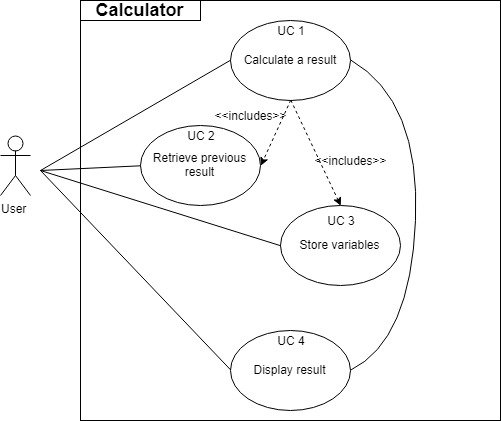
\includegraphics[width=0.4\linewidth]{UseCaseDiagram.jpg}
        \end{tikzfigure}
        
        \vspace{10mm}
         
         Users had very differing demands but we were able to extract commonalities to arrive at goals/use cases.
         
         \vspace{5mm}
         
         \begin{itemize}
         \item Technical/Mathematical: Access to advanced functions, precision, mapping keys to functions to customize.
        \item Common/Casual User: Simple functions, simple looking, portability.
        \item Academic User: Key mapping for personalisation and easy access to key functions.
         \end{itemize}
    }
   

    \column{0.36}
    \block{What's Inside?}{
       
       Following from the requirements gathering, we decided to include the following features which align with the user requirements and satisfy the use cases.
       
       \vspace{10mm}
       \textbf{Feature List:}
        \vspace{5mm}
         \begin{itemize}[leftmargin=0.7in]
             \item Type expressions in natural language (Simplicity)
             \item Define constants (Customizable)
             \item Recall previous result (Reliability, Simplicity)
             \item View complete calculation history (Reliability, Simplicity)
             \item Different themes (Customizable)
             \item Visual feedback with detailed error messages (Reliability, Simplicity)
         \end{itemize}
         \vspace{5mm}
        
        
        \vspace{1em}
        \begin{tikzfigure}[Calculator with example calculations]
            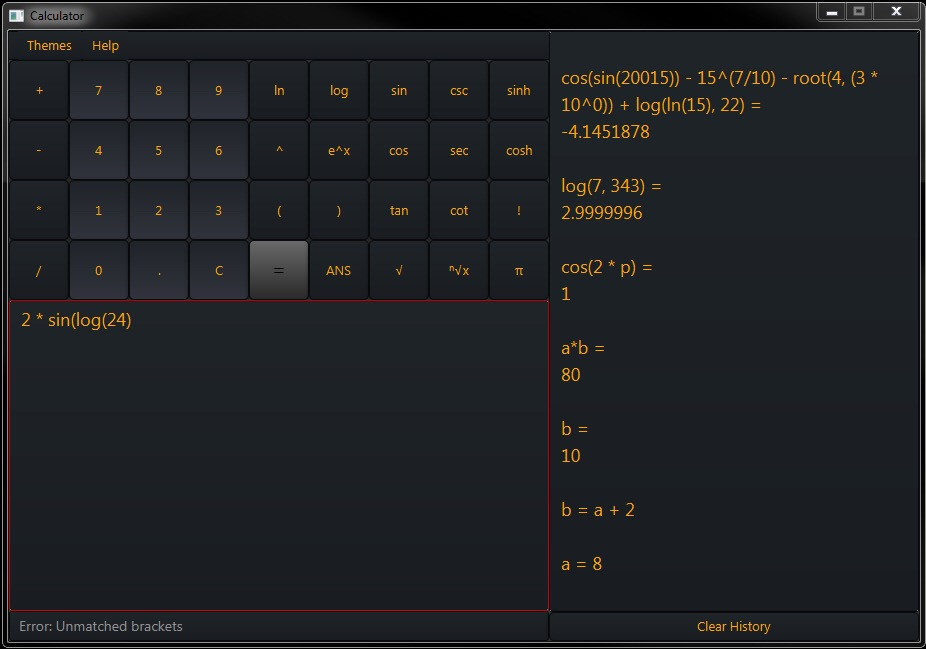
\includegraphics[width=0.9\linewidth]{Calculator.jpg}
        \end{tikzfigure}
        \vspace{1em}
        
        \textbf{User Experience}
        \begin{itemize}[leftmargin=0.7]
            \item Input box place to encourage user to type in expression and reduce reliance on buttons.
            \item Buttons placed in a way to easily reach the most commonly used functions.
            \item left side is where use interacts with the controller where as the right side is where he/she sees the view (i.e. MVC pattern)
        \end{itemize}
        
    }
    
    \column{0.32}
    \block{Solution}{
    
    \begin{itemize}[leftmargin=0.7in]
        \item \textbf{Technical/Mathematical:} Access to advanced functions, precision, mapping keys to functions to customize. (feels like they can program the calculator to their liking)
        \item \textbf{Common/Casual User:} Simple functions, simple looking, portability.
        \item \textbf{Academic User:} Key mapping for personalisation and accessing key functions for courses in a simple way.
    \end{itemize}
        \begin{tikzfigure}[Light Theme Calculator]
            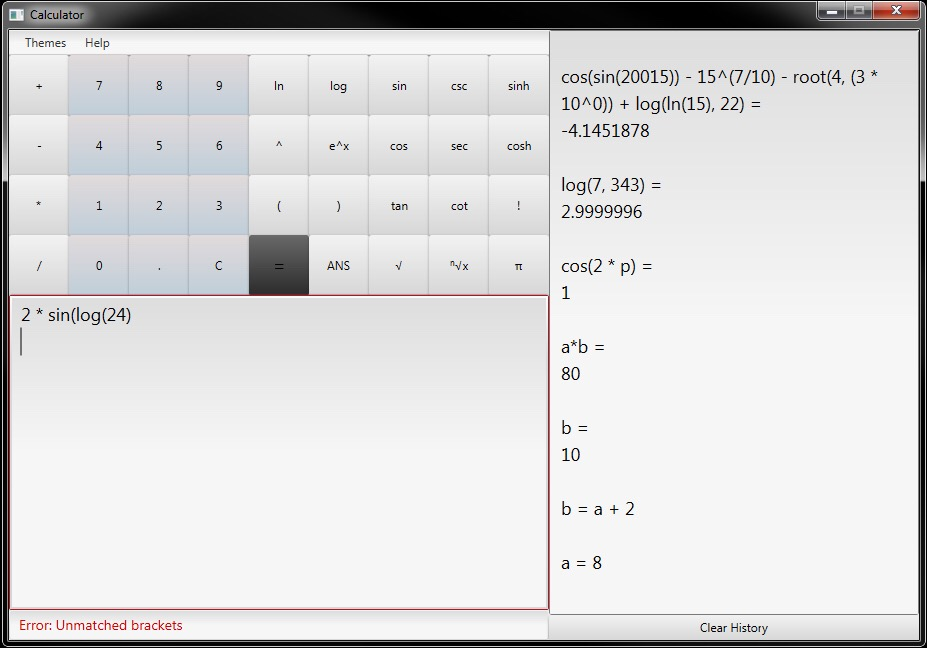
\includegraphics[width=0.4\linewidth]{CalculatorLight.jpg}
        \end{tikzfigure}
    }
    
    \block{Challenges}{
         Some of the obstacles we faced were simple, while others were so challenging that they made us reconsider our architecture:
         
        \vspace{5mm}
        \begin{itemize}[leftmargin=0.7in]
            \item inaccuracies in the power function due to the exponential growth of slight offsets
            \item Large numbers in power function and root function resulted in stalls due to large number of iterations.
            \item In rare cases, user can enter input that may result in undefined behavior.
        \end{itemize}
        \vspace{5mm}
    }
    
    \block{Future}{
     Main focus is on UX (user experience) to create an engaging, portable, and personalized tactile experience!
     
    \begin{itemize}[leftmargin=0.7in]
        \item Improving the overall UX experience (themes, keymapping)
        \item Making our calculator available online 
        Accessible on different platforms (e.g. smartphones)
        \item Continued Maintenance on Code (Code architecture for ease of maintenance and modification)
    \end{itemize}

    }
\end{columns}
\end{document}